\documentclass[oneside,a4paper,spanish,links]{amca}
%
\usepackage{graphicx}
\usepackage{amsmath,amsfonts}
\usepackage[utf8]{inputenc}
%
\title{PREPARACIÓN Y SIMULACIÓN DE CASO 3D EN OPENFOAM}
%
\englishtitle{SETUP AND SIMULATION OF 3D CASE IN OPENFOAM}

\author[a]{Guillermo Rolle}
%\author[b]{Segundo B. Autor}
%\author[b]{Tercer C. Autor}
%\author[a]{Cuarto D. Autor}
%
%\affil[a]{Grupo de Mecánica Computacional, Universidad Nacional de
%Villa Carolina, Los Alerces 3492, 4200~Villa Carolina, Argentina,
%gmc@uncarolina.edu.ar, \url{http://www.uncarolina.edu.ar/gmc}}
%
%\affil[b]{Grupo de Ingeniería Aplicada, Universidad Nacional de La
%Meseta, Los Cipreses 3493, 4201~La Meseta, Argentina,
%gia@unmeseta.edu.ar, \url{http://www.unmeseta.edu.ar/gia}}

%% NOTA: SI TODOS LOS AUTORES TIENEN LA MISMA AFILICACION
%% USE EL MACRO `\voidaffil' PARA EL CODIGO DE AFILICACION.
%% Ejemplo:
%% \author[\voidaffil]{Primer A. Autor}
%% \author[\voidaffil]{Segundo B. Autor}
%% \author[\voidaffil]{Tercer C. Autor}
%% \author[\voidaffil]{Cuarto D. Autor}
%% %
%% \affil[\voidaffil]{Grupo de Mecánica Computacional,
%% Universidad Nacional de Villa Carolina,
%% Los Alerces 3492, 4200 Villa Carolina, Argentina,
%% gmc@uncarolina.edu.ar, http://www.uncarolina.edu.ar/gmc}

\begin{document}
\vspace{3cm}

\maketitle

%% To set PDF METADATA: uncomment and replace fields in
%% UPPERCASE with appropriate values.
%%
%% \hypersetup{
%%   pdfauthor={AUTHORS},
%%   pdfkeywords={KEYWORDS},
%%   pdftitle={TITLE}
%% }
%%
%% For instance
%% \hypersetup{
%%   pdfauthor={Sponge B. and Star P.},
%%   pdfkeywords={multiphase flow, air-liquid mixtures},
%%   pdftitle={A new model for multi-phase flow}
%% }
%%
%% NOTE: To set the metadata is recommended but not absolutely
%% neccesary.
%% This was done before with the \pdfinfo command,
%% but according to this post:
%% http://de.nntp2http.com/comp/text/tex/2008/12/5358fd061de9703a781885a5dcf98364.html
%% if `hyperref' is used, then you must use \hypersetup{} not \pdfinfo{}

\begin{keywords}
CFD, OpenFOAM, FreeCAD, simpleFoam, scalarTransportFoam
\end{keywords}

\begin{abstract}
Este documento provee información e instrucciones para realizar una simulación de un caso 3D en OpenFOAM.
La geometría 3D se modela con software FreeCAD y se malla con snappyHexMesh. Luego, se ejecutan las simulaciones correspondientes con simpleFoam y scalarTransportFoam.  Se mantienen las condiciones de contorno e iniciales de los informes anteriores. El documento finaliza con conclusiones sobre el caso y los resultados obtenidos. \\
%
\linebreak
%
\textbf{Keywords:} CFD, OpenFOAM, FreeCAD, simpleFoam, scalarTransportFoam\\
%
\linebreak
%
\textbf{Abstract.} This document provides information and
instructions to setup a 3D OpenFOAM case. The geometry is defined with FreeCAD software and is meshed with snappyHexMesh. Afterwards, the corresponding simulations will be run using solvers simpleFoam and scalarTransportFoam. Initial conditions and boundary conditions are kept from previous reports. The document ends with conclusions about the case and the results obtained.
%\\
%\\
%\textbf{Agradecimientos:} Los autores agradecen... (no más de 2 líneas)
% LOS AGRADECIMIENTOS EN LA PRIMERA PAGINA SE PERMITEN SOLO PARA
% PRESENTACIONES DE RESUMENES (NO PARA ARTICULOS COMPLETOS)
\end{abstract}

\section{INTRODUCCIÓN}
En este documento se detallan los pasos a seguir para preparar y ejecutar una simulación en 3 dimensiones con OpenFOAM (ver figura \ref{fg:intro}). Se modela la geometría con software FreeCAD. El caso descrito en este informe se puede descargar del repositorio público: \url{https://github.com/guillerolle/casos_cfd/tree/master/03}. En el repositorio se encuentran también los archivos para FreeCAD.

Se asume que el lector tiene una versión de FreeCAD disponible y lista para utilizar en conjunto con OpenFOAM. No se hará demasiado hincapié en el modelado de la geometría, sino más bien en todo lo que implique a OpenFOAM y CFD en sí.

\begin{figure*}[htb]
	\centerline{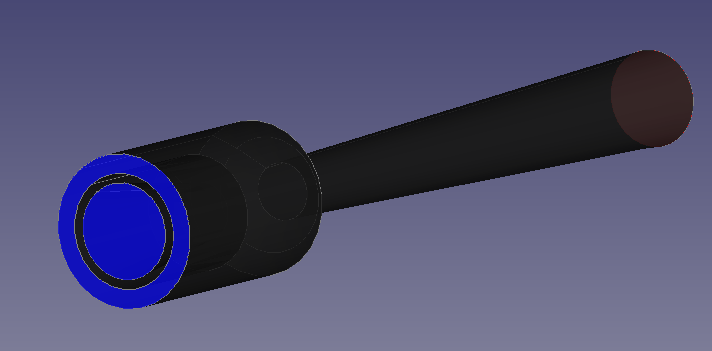
\includegraphics[width=0.8\textwidth]{Figuras/01_INTRO.png}} \caption{Caso 3D en cuestión} \label{fg:intro}
\end{figure*}

Este informe es parte de la serie de informes de \url{https://github.com/guillerolle/informes_cfd}. Estos casos están basados en un mezclador de agroquímicos en línea.

\section{PREPARACIÓN DE LA GEOMETRÍA}
El primer paso es realizar el modelo en FreeCAD del espacio de fluido que usaremos en la simulación. Es decir, nuestro volumen de control (macroscópicamente). En la figura \ref{fg:boceto_revo} se muestra el boceto del modelo. 

\begin{figure*}[htb]
	\centerline{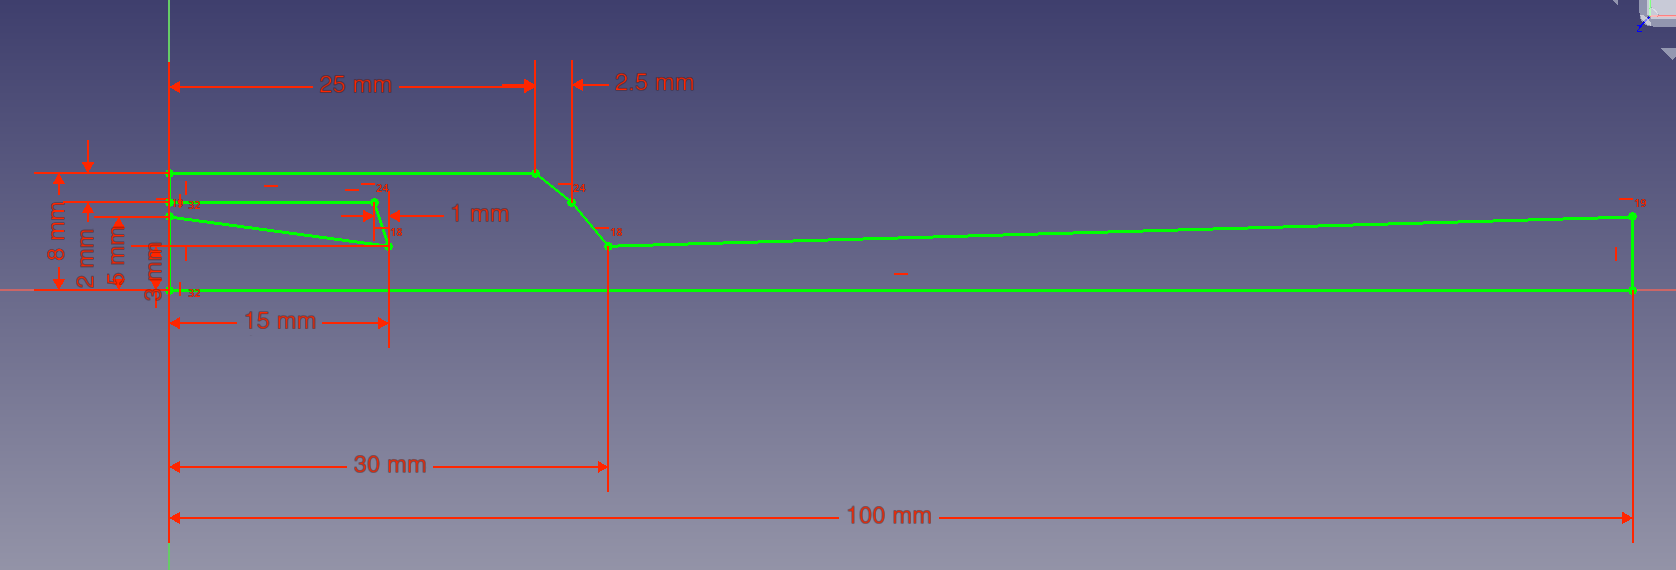
\includegraphics[width=0.8\textwidth]{Figuras/02_BOCETO_REVOLUCION.png}} \caption{Croquis de la geometría} \label{fg:boceto_revo}
\end{figure*}

Haciendo una revolución de este croquis sobre el eje inferior, obtenemos la geometría en cuestión y podemos empezar a preparar el caso de CFD.

\begin{figure*}[htb]
	\centerline{
\includegraphics[width=0.8\textwidth]{Figuras/02_BOTONES_CFD.png}} \caption{Acciones disponibles en espacio de trabajo \textbf{CfdOf}} \label{fg:botones_cfd}
\end{figure*}

En el espacio de trabajo \textbf{CfdOf} iniciaremos un nuevo estudio de CFD. Al iniciar el estudio, se habilitarán los botones de CFD en la barra superior (ver figura \ref{fg:botones_cfd}).

Antes de empezar, debemos definir la ruta de salida para el caso de OpenFOAM. Es decir, qué directorio utilizara FreeCAD para ejecutar las simulaciones. En la figura \ref{fg:fc_outputpath} se muestra dónde puede modificarse ésta ruta.

\begin{figure*}[htb]
	\centerline{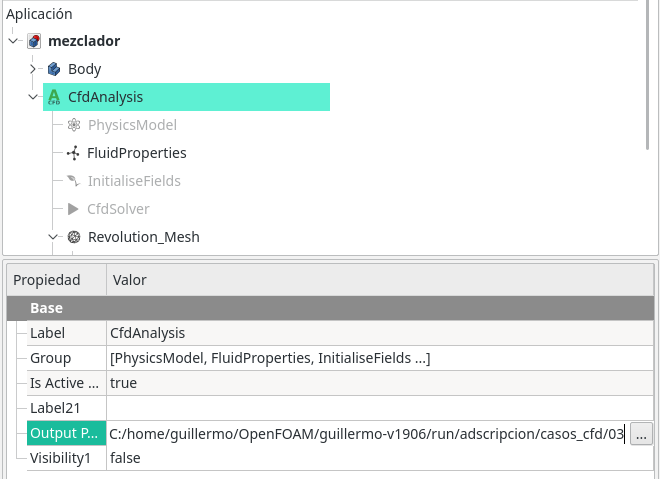
\includegraphics[width=0.7\textwidth]{Figuras/02_OUTPUTPATH.png}} \caption{Propiedad \textit{Output Path} en \textit{CfdAnalysis}} \label{fg:fc_outputpath}
\end{figure*}



Definimos las condiciones de contorno para cada cara de la geometría y ajustamos las propiedas del fluido y del solver. Ver las condiciones y propiedades correspondientes en los archivos del \href{https://github.com/guillerolle/casos_cfd/tree/master/03}{repositorio}. Una vez hecho esto tendremos un árbol similar a la de la figura \ref{fg:estructura_freecad}.

\begin{figure*}[htb]
	\centerline{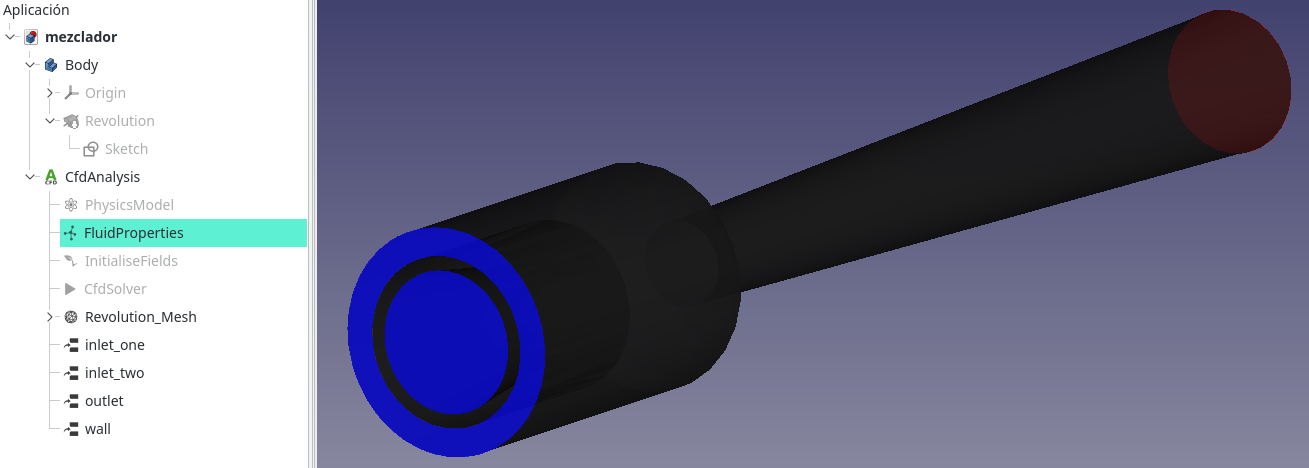
\includegraphics[width=0.7\textwidth]{Figuras/02_ESTRUCTURA_FREECAD.png}} \caption{Estructura básica del estudio CFD} \label{fg:estructura_freecad}
\end{figure*}

\subsection{Mallado}
Seleccionamos el sólido de revolución y elegimos la opción de crear una nueva malla a partir del sólido. Usamos el mallador \textbf{snappyHexMesh} en \textbf{3D} y un tamaño base de elemento 0.5mm. Usamos la utilidad para encontrar un punto dentro de la geometría y cerramos la ventana de tareas (todavía no ejecutar el caso de mallado). Vamos a crear además un refinamiento sobre las superficies de las paredes para tener una mejor definición de la capa límite. Para esto, seleccionar la malla (en el estudio CFD) y clickear en refinamiento de malla. Seleccionamos refinamiento por superficie y tamaño relativo de 0.5. Luego seleccionamos todas las superficies de pared.

Con esto estamos listo para escribir el caso de mallado y ejecutarlo. En la figura \ref{fg:pv_malla} se muestra la malla generada en el visualizador \textbf{ParaView}. Observar el refinamiento sobre las paredes. Tener en cuenta que \textbf{Paraview} presenta algunos errores en la visualización de la malla, pero el mallado es correcto. Comprobar ejecutando \texttt{checkMesh}. También corroborar que las regiones de entrada/salida estén definidas correctamente.

\begin{figure*}[htb]
	\centerline{
		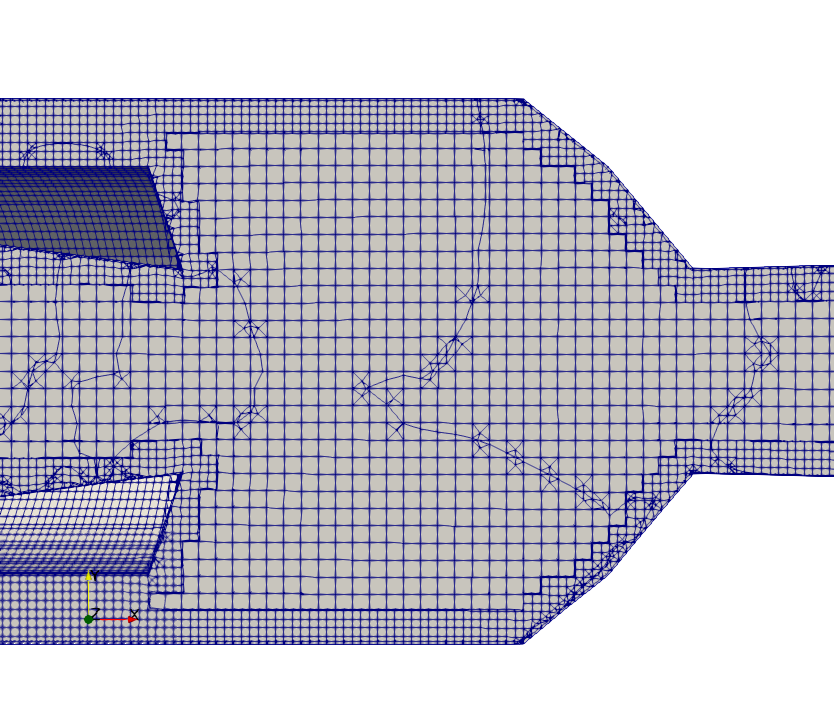
\includegraphics[width=0.4\textwidth]{Figuras/02_MALLA_CAMARA.png}
		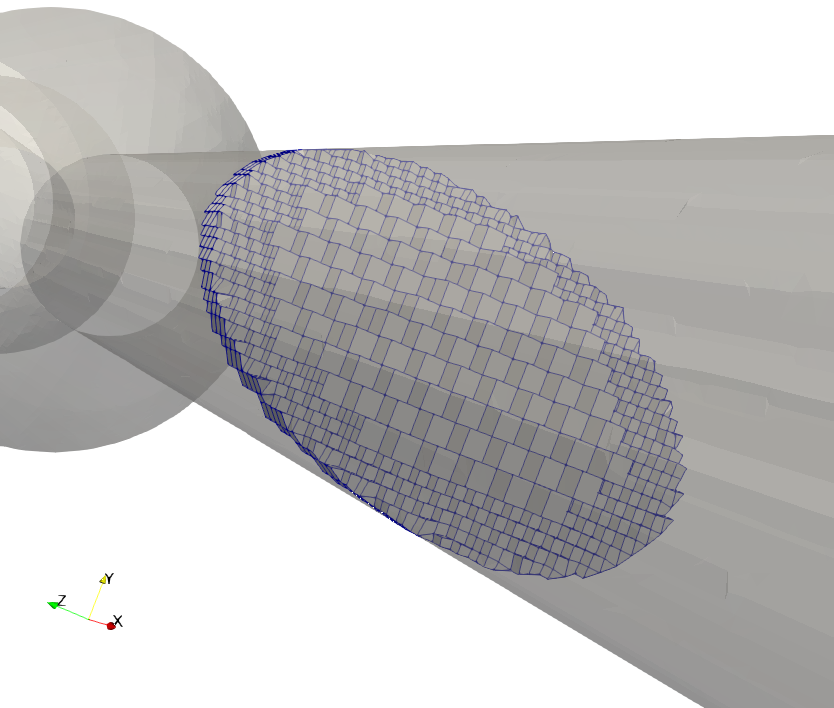
\includegraphics[width=0.4\textwidth]{Figuras/02_MALLA_SECCION.png}} \caption{Malla en cámara de mezcla (izquierda) y en sección interna del difusor de salida (derecha)} \label{fg:pv_malla}
\end{figure*}

\newpage
\section{SIMULACIÓN SIMPLEFOAM}
Una vez creada la malla y definidas las propiedas del solver (modelo estacionario, flujo incompresible, agua, etc.) abrimos la sección \textbf{CfdSolver} en \textbf{FreeCAD} y escribimos el caso. Antes de ejecutarlo, debemos realizar algunas modificaciones en los archivos \textit{fvSolution} y \textit{fvSchemes}. En el repositorio se encuentran los archivos \href{https://github.com/guillerolle/casos_cfd/tree/master/03/case/system/fvSolution.bkp}{fvSolution.bkp} y \href{https://github.com/guillerolle/casos_cfd/tree/master/03/case/system/fvSchemes.bkp}{fvSchemes.bkp}. Reemplazar los anteriores por éstos últimos para mejorar la convergencia de la simulación.

Se sugiere utilizar una utilidad como \href{https://meldmerge.org}{Meld} para comparar archivos y/o carpetas. En la figura \ref{fg:meld} se muestra esta utilidad comparando los archivos mencionados.

\begin{figure*}[htb]
	\centerline{
		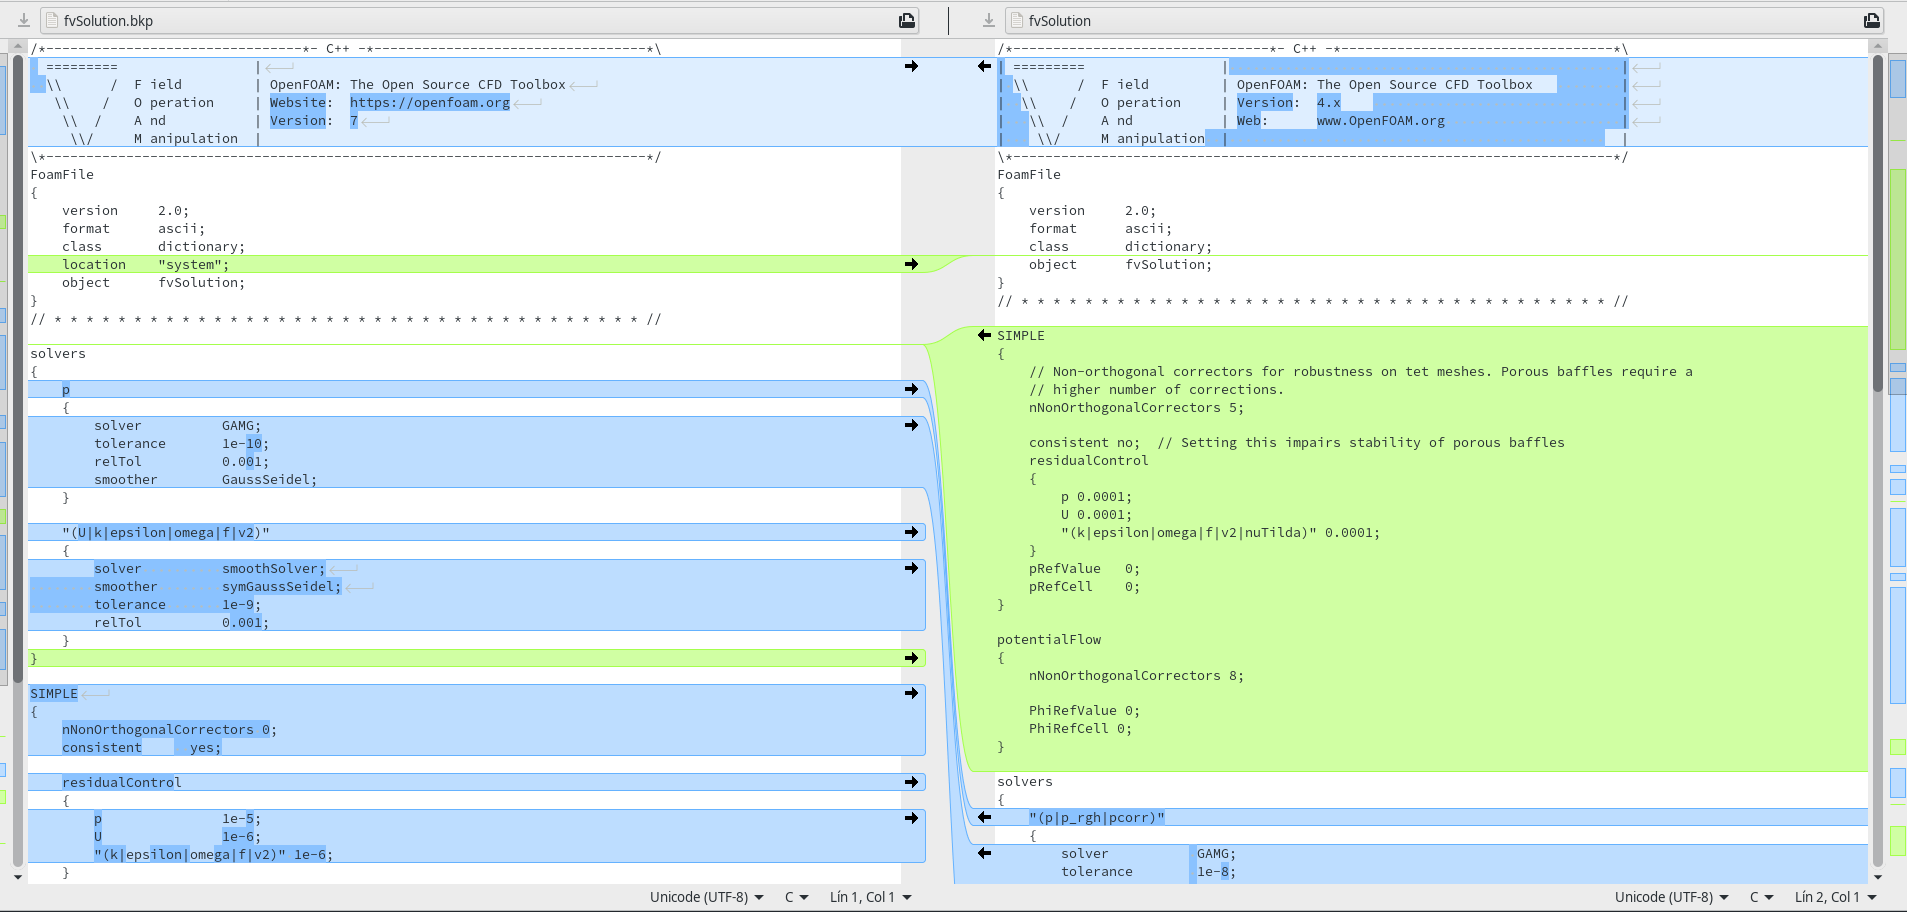
\includegraphics[width=0.8\textwidth]{Figuras/03_MELD.png}}
		 \caption{Comparación archivos fvSolution.bkp (izquierda) con fvSolution (derecha)} \label{fg:meld}
\end{figure*}

Volviendo a FreeCAD, podremos ejecutar la simulación con \textit{RUN}. Observar que la evolución de los residuales (figura \ref{fg:03_sf_residuales}) comienza a oscilar sobre un valor aproximadamente constante a partir de la iteración número 1000 sin llegar nunca a las tolerancias definidas en \textit{system/fvSolution}. 

\begin{figure*}[htb]
	\centerline{
		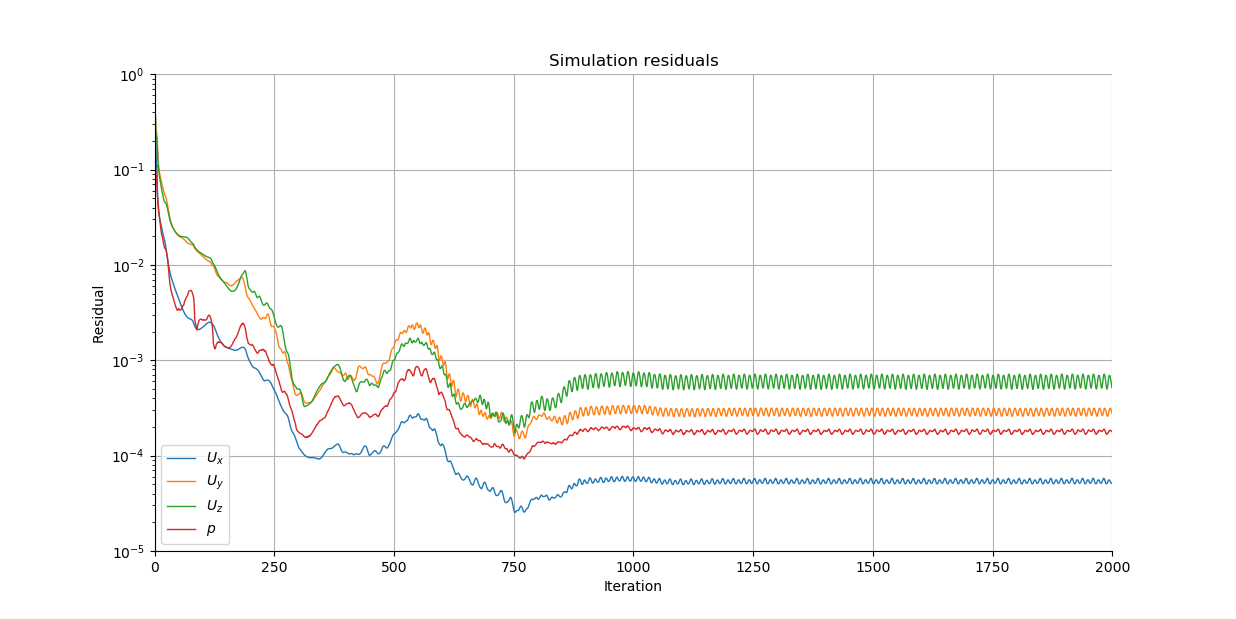
\includegraphics[width=0.8\textwidth]{Figuras/03_SF_RESIDUALES.png}}
	\caption{Evolución de residuales con simpleFoam} \label{fg:03_sf_residuales}
\end{figure*}

Sin necesidad de esperar a que termine de correr la simulación, podemos ver la evolución del perfil en ParaView. En la figura \ref{fg:03_sf_U} se muestra el campo de velocidades para una iteración bastante avanzada de la simulación (1700). Al comparar con pasos de tiempo consecutivos, no se aprecian grandes diferencias en los campos de velocidad o presión, por lo que asumiremos que la simulación fue satisfactoria.
FreeCAD descompone el caso en varios procesadores, por lo que para ver los resultados en ParaView debemos seleccionar "DecomposedCase".

\begin{figure*}[htb]
	\centerline{
		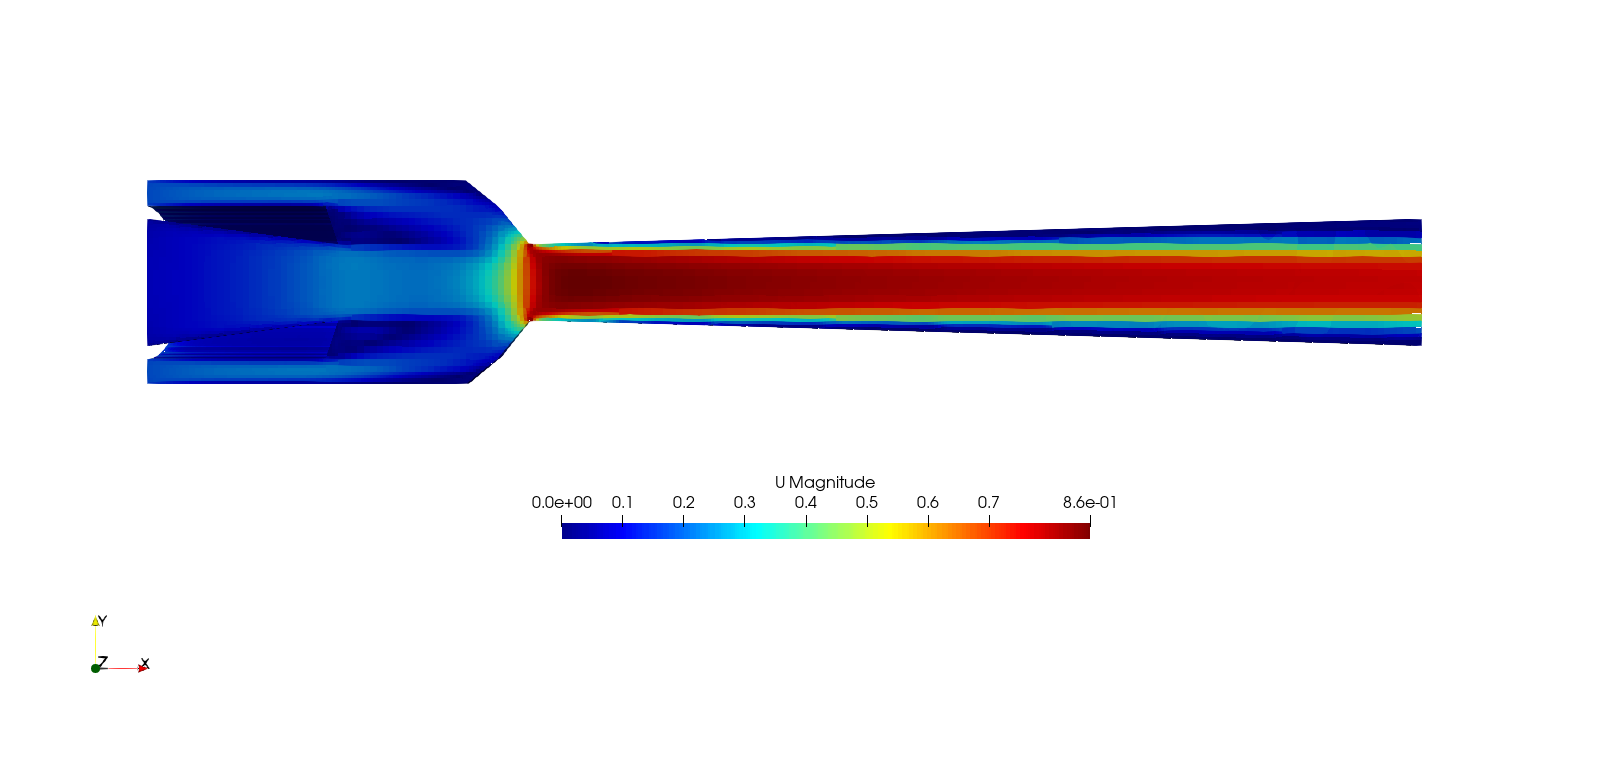
\includegraphics[width=0.8\textwidth]{Figuras/03_SF_U.png}}
	\caption{Campo de velocidad U obtenido} \label{fg:03_sf_U}
\end{figure*}

\subsection{Reconstrucción del caso}
Ya sabemos de los informes anteriores que necesitamos copiar el campo de presión y velocidad obtenidos con esta simulación en otro directorio que contenga el caso de la simulación RTD. Como el caso fue ejecutado en varios procesadores, en el directorio principal no encontraremos los pasos de simulación. Éstos se encuentran en las carpetas \texttt{processor*} y los archivos están divididos (caso descompuesto).

Para reconstruir el caso debemos ejecutar el comando \texttt{\$ reconstructPar} en el directorio \textit{case}. Ahora encontraremos los campos de presión y velocidad para la iteración 2000 en el directorio principal.

\section{SIMULACIÓN SCALARTRANSPORTFOAM}


\section{ESPECIFICACIONES GENERALES}

El artículo puede ser escrito en inglés, español o portugués
dentro de una caja de impresión de 16cm x 24cm, centrada en la
página. El documento, incluyendo figuras, tablas y referencias,
deben tener una longitud mínima de 4 páginas y no debe exceder las
10 páginas. El documento debe ser cargado en el sitio de AMCA como
archivo en formato \textbf {PDF}; no se aceptan otros formatos (MS
Word, RTF). El tamaño del archivo PDF del documento no debe
Exceder 2~MBytes.

\subsection{Uso de acrónimos}

Si se usan acrónimos, entonces debe definirlos antes de su primer ocurrencia.

\section{TÍTULO, AUTORES, AFILIACIÓN, PALABRAS CLAVE}

La primera página debe contener el Título, Autor(es),
Afiliación(es), Palabras clave y el resumen. Si el idioma elegido
es el español o el portugués, se debe agregar el duplicado del
título, palabras clave y resumen en inglés, siguiendo como ejemplo
el presente instructivo. La segunda página debe comenzar con la
Introducción. La primera línea del título se encuentra a 3cm de la
parte superior de la caja de impresión para agregar el membrete
AMCA.

\subsection{Título}

El título se debe escribir centrado, con 14pt, en Times Roman
negrita y todas las letras en mayúsculas. Debe tener espaciado
simple si el título tiene más de una línea de longitud. \textbf{No
se recomienda} la inclusión de fórmulas o caracteres especiales en
el título. Se pueden utilizar acrónimos si se definen \emph{en
línea}, por ejemplo ``flujo alrededor de un cilindro utilizando
Large Eddy Simulation (LES)''. La traducción al inglés del título
se debe escribir centrada, con 12pt, en Times Roman negrita y
todas las letras en mayúsculas.

\subsection{Autor}

El nombre del autor debe incluir el nombre, la inicial del segundo
nombre y el apellido. Debe estar escrito centrado, en 12pt,
negrita, Times Roman, a 12pt debajo del título. Ubique a todos los
autores juntos, divididos en varias líneas si fuese necesario.
Antes del último autor debe estar el conector ``{\bf y}''. Las
afiliaciones deben estar organizadas en bloques centrados, después
de los autores. Identifique a cada autor con su correspondiente
afiliación usando un superíndice como en el ejemplo. Si todos los
autores pertenecen a la misma afiliación no utilice superíndice.

\subsection{Afiliación}

La afiliación del autor se debe escribir centrada, en 11pt, en
Times Roman itálica, a 12pt debajo de la lista de autores. Un
espacio de 12pt debe separar dos afiliaciones distintas. Se
recomienda que los autores incluyan, en lo posible, su dirección
de correo electrónico y una página web por sitio de afiliación.

\subsection{Palabras clave}

Por favor, escriba a lo sumo seis palabras clave. Deben escribirse
alineadas a la izquierda, en 12pt Times Roman, y la línea debe
comenzar en fuente negrita con {\bf Palabras Clave}. Un espacio de
12pt debe separar las palabras clave del texto de las
afiliaciones. Utilice la palabra {\bf Keywords} para encabezar la
traducción al inglés de las palabras clave. Un espacio de 12pt
debe separar las palabras clave del texto del resumen en español.

\subsection{Resumen}

Utilice fuente Times Roman de 11pt para el resumen. El resumen
debe tener un párrafo único sin saltos de línea. La palabra
\textbf{Resumen} debe estar en negrita al principio de la primera
línea. El texto del resumen debe estar justificado y separado 12pt
como se muestra en la primera página de estas instrucciones. El
resumen debe ser autónomo, por lo que no se deben incluir figuras,
tablas o ecuaciones. Tampoco se deben incluir referencias cruzadas
a tales materiales. Se desaconseja incluir referencias a otros
trabajos en el resumen. En caso de incluirse referencias, deben
hacerse \emph{en línea}, pero en forma abreviada como en este
ejemplo (C. Jhonson et al., \emph{Int J Num Meth Eng},
34(3):543--568 (1992); D. Mitchell y J. Brady, \emph{J Sound Vib},
21(2):221--230 (2006)). Las citaciones múltiples deben separarse
por punto y coma. \textbf{No se recomienda incluir más de 2
referencias en el resumen}. Evite incluir caracteres especiales y
fórmulas. Si utiliza acrónimos, debe definirlos inmediatamente
antes de su primera ocurrencia. Ubique la traducción al inglés del
resumen separándolo un espacio de 12pt de la traducción de las
palabras clave; debe estar encabezado por la palabra
\textbf{Abstract} en negrita. Se sugiere una extensión del resumen
entre 150 y 300 palabras considerando que con las traducciones en
inglés quede todo contenido en la primer página.

\section{TÍTULOS EN EL TEXTO}

\subsection{Títulos principales}

Los títulos principales se deben escribir alineados a la
izquierda, en 12pt, en Times Roman negrita, con letras todas
mayúsculas. Debe haber un espacio de 12pt antes y de 6pt después
de los títulos principales.

\subsection{Títulos secundarios}

Los títulos secundarios deben ser escritos alineados a la
izquierda, en 12pt, en Times Roman negrita, con una mayúscula en
la letra inicial para la primera palabra solamente. Debe haber un
espacio de 12pt antes y de 6pt después de los títulos secundarios.

\section{TEXTO}

El texto normal debe escribirse con espaciado simple, justificado,
utilizando fuente de 12pt Times Roman, en una columna. La primera
línea de cada párrafo debe tener una sangría de 0,5cm. No debe
haber separación entre párrafos.

\section{NÚMEROS DE PÁGINA}

Los autores {\bf no deben numerar} las páginas del artículo. Los
números serán agregados por el editor.

\section{FIGURAS}

Todas las figuras deben numerarse consecutivamente y tener su
leyenda o subtítulo. El subtítulo se debe escribir centrado, en
10pt Times Roman, en minúsculas con letra mayúscula para la primer
letra de la oración.

\begin{figure*}[htb]
\centerline{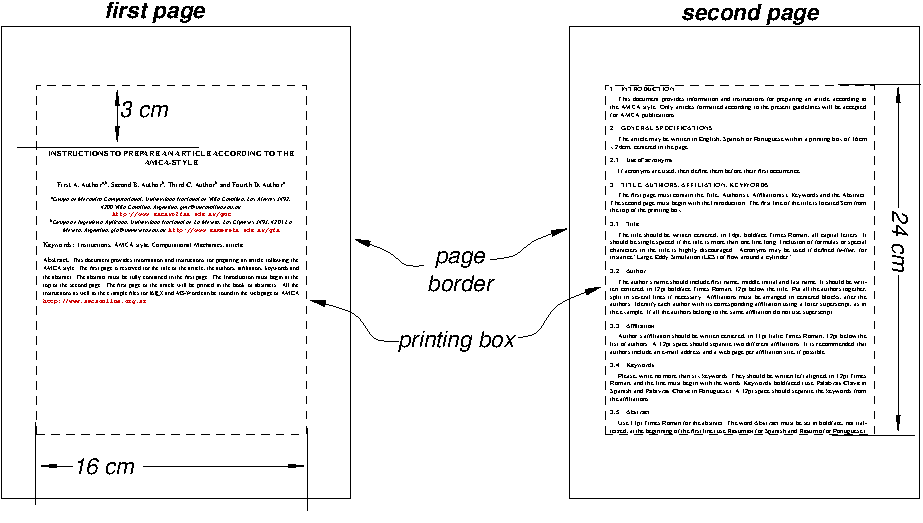
\includegraphics{firstpage}} \caption{Disposición de
la página.} \label{fg:figura}
\end{figure*}

Un espacio de 6pt debe separar la figura de su leyenda, y un 12pt
espacio debe separar el texto que la rodea de la parte superior de
la figura y de la inferior de la leyenda (véase la
Fig.~\ref{fg:figura}).

Todas las figuras deben estar referenciadas en el texto. Las
figuras en color son bienvenidas.

\section{ECUACIONES}

Cada ecuación debe estar numerada utilizando números arábigos
entre paréntesis. Debe estar centrada, dejando un espacio de 6pt
arriba y abajo para separarla del texto que la rodea.

El ejemplo siguiente es una ecuación de línea simple
%
\begin{equation}
Ax = b.
\end{equation}

El ejemplo siguiente es una ecuación de varias líneas
%
\begin{equation} \label{eq:simple}
\begin{aligned}
Ax& = b,\\
Ax& = c.
\end{aligned}
\end{equation}
%
En lo posible, se deben generar los vínculos internos del PDF para
las referencias a las ecuaciones. El color recomendado para los
vínculos a referencias en el texto es el azul; por ejemplo, ver
Ec.~(\ref{eq:simple}).

\section{TABLAS}

Todas las tablas deben estar numeradas y tener su descripción.
Esta descripción debe tener tamaño 10pt y fuente Times Roman, con
letras minúsculas y mayúscula en la primera letra de la oración.

Un espacio de 6pt separa la tabla de la descripción, y un espacio de 12pt
separa la tabla del texto que la rodea. Por ejemplo, ver la
Tabla~\ref{tab:n50}. Todas las tablas deben estar referencias en el texto.

\begin{table}[htb]
\centering
\begin{tabular}{|c|c|c|c|}
\hline  & malla 20x20  & malla 50x50  & malla 100x100 \\
\hline
\hline
 0 & 41,00 & 1.00 & 4,92\\
\hline
 1 & 40,86 & 1.02 & 4,88 \\
\hline
10 & 23,81 & 3,44 & 2,92 \\
\hline
50 & 5,62 & 64,20 & 1,08 \\
\hline
\end{tabular}
\caption{Número de condición para el operador de Stekhlov.}
\label{tab:n50}
\end{table}

\section{FORMATO DE  REFERENCIAS}

Las referencias deben insertarse en el texto utilizando el estilo
\emph{autor-fecha} (también conocido como \emph{Harvard style}).
Las referencias se pueden citar entre \emph{paréntesis} como
\citep{zienkiewicz91,idelsohn94,meyer82,meyer82b},
 o en forma \emph{textual}, por ejemplo, ver
\citet{zienkiewicz91,idelsohn94,meyer82,meyer82b}. Las referencias
deben agruparse y ordenarse alfabéticamente al final del artículo
como se muestra en estas instrucciones. No incluya referencias que
no sean citadas en el cuerpo del artículo. Utilice referencias con
símbolos Romanos; no utilice, por ejemplo, símbolos griegos,
chinos o japoneses.

En lo posible, debe generar los vínculos internos dentro del PDF para las citaciones.
El color recomendado para los vínculos a referencias en el texto es el azul.
El color preferido para vínculos a referencias externas, como las páginas web,
 es el rojo (por ejemplo, \url{http://www.amcaonline.org.ar}).

\section{CONCLUSIONES}

Los archivos fuente en TeX, \LaTeX{} y ejemplos en MS-Word se
pueden encontrar en el sitio web de AMCA:
\url{http://www.amcaonline.org.ar}. Se recomienda el uso de estos archivos para respetar el formato con mayor facilidad. Recuerde: {\bf No numere las
páginas.}

%\section*{AGRADECIMIENTOS} Los autores agradecen a ...
% ACKNOWLEDGEMENTS FOR FULL ARTICLES
%
\bibliography{amcapaper}
\end{document}
